% ----------------------------------------

\subsection{Environment behavior}

% ----------------------------------------

\begin{frame}
\frametitle{Non-stationary behavior}
\framesubtitle{Overview}

By using the \textbf{non-stationarity} assumption we are taking into consideration that the demand curve could be subject to changes over time and isn't necessarily fixed as we have seen in other steps.

There are 2 main types of \textit{non-stationary behaviors}:
\begin{itemize}[label={$\circ$}]
    \item \textbf{Abrupt changes}: where it's possible to identify different phases with different phase-wise stationary demand curves.
    \item \textbf{Smooth changes}: where the demand curve changes over time in a continuous manner.
\end{itemize}

As per specifications, we will only consider \textbf{abrupt changes} in the scope of our project.

\end{frame}

% ----------------------------------------

\begin{frame}
\frametitle{Non-stationary behavior}
\framesubtitle{Abrupt changes}

\textbf{Abrupt changes} are usually experienced when an important event strikes the market \textit{(e.g. a new product that shifts the interests of the users is released or an historical event shapes the opionion of people)}; change isn't necessarily bad, however, it may impact negatively the prediction of learners that were created with a static environment in mind.

Neither \textbf{UCB} nor \textbf{TS} account for abrupt changes since it's almost impossible for them to try a superarm that was deemed as \textit{unoptimal} over the past iterations (while it might have become optimal after an \textit{abrupt change}), therefore we expect to see a significant \textbf{reward drop} from them after an \textit{abrupt change}.

\end{frame}

% ----------------------------------------

\subsection{Algorithms}

% ----------------------------------------

\begin{frame}
\frametitle{Approaches}
\framesubtitle{Sliding window and Change detection}

There are 2 main approaches to deal with a \textbf{non-stationary environment}
\begin{itemize}[label={$\circ$}]
    \item \textbf{Sliding window}: only consider the last $\tau$ samples for predictions.
    \item \textbf{Change detection}: detect when a change has happened and adapt accordingly.
\end{itemize}

It's clear that \textbf{Sliding window} approaches are more fit for \textbf{smooth changes} while \textbf{Change detection} approaches work better with \textbf{abrupt changes}, however it's important to note that both approaches can be utilized to deal with any \textit{non-stationary} scenario.

\end{frame}

% ----------------------------------------

\begin{frame}
\frametitle{Sliding window}
\framesubtitle{Sliding window for TS and UCB}

\begin{itemize}[leftmargin=*, label={$\circ$}]
    \item \textbf{SW-GPTS} only differs in the \textbf{gaussian process} update since the older samples are progressively removed from the estimation as time goes on.
    \item \textbf{SW-GPUCB} also differs in the confidence bound formulation and the new arm choice:
        \begin{displaymath}
            a_t =
            \begin{cases}
                a_{\overline{t}} & \text{if} ~ \exists \overline{t} ~ | ~ n_{a_{\overline{t}}}(t-1, \tau) = 0 \\
                arg\max_{a \in A} \left\{ \mu_{t-1, \tau} + \delta \sigma_{t-1, \tau} \right\} & \text{otherwise}
            \end{cases}
        \end{displaymath}
\end{itemize}

\end{frame}

% ----------------------------------------

\begin{frame}
\frametitle{Change detection}

We used a \textbf{reward-based algorithm} as a \textit{change detection algorithm}, it works by comparing the last $k$ rewards with the newest $k$ rewards ($k=4$ by default) and if the difference between their means exceedes a certain threshold $\omega$ ($\omega=1000$ by default) the learner is \textbf{reset} and is therefore able to learn a new optimal superarm from scratch.

Formally:
\begin{displaymath}
    \text{RESET learner if} ~ t \geq 2k ~ \land \sum_{i=t-2k}^{t-k} r_i -\sum_{i=t-k+1}^t r_i > \omega
\end{displaymath}

\scriptsize N.B. there is an offset of 1 in the representation of t between theory and code

\end{frame}

% ----------------------------------------

\subsection{Results}

% ----------------------------------------

\begin{frame}[plain]

\frametitle{Average reward and regret}
\framesubtitle{Base learner}

\begin{center}
    \hspace*{-2.8em}
    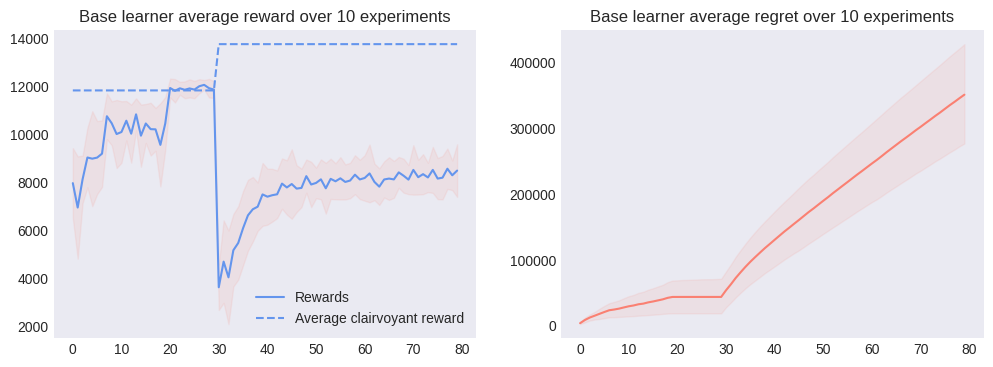
\includegraphics[scale=0.5]{img/Graphs/non_stationary/image1.png}
\end{center}

\end{frame}

% ----------------------------------------

\begin{frame}[plain]

\frametitle{Average reward and regret}
\framesubtitle{Sliding window}

\begin{center}
    \hspace*{-2.8em}
    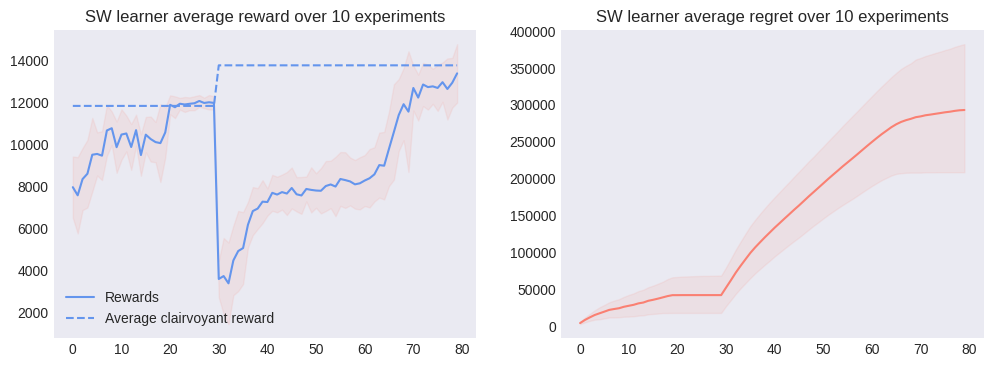
\includegraphics[scale=0.5]{img/Graphs/non_stationary/image2.png}
\end{center}

\end{frame}

% ----------------------------------------

\begin{frame}[plain]

\frametitle{Average reward and regret}
\framesubtitle{Change detection}

\begin{center}
    \hspace*{-2.8em}
    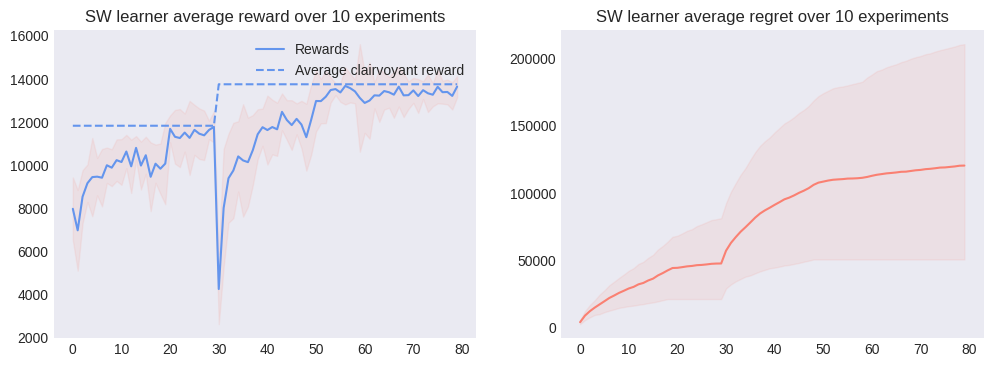
\includegraphics[scale=0.5]{img/Graphs/non_stationary/image3.png}
\end{center}

\end{frame}

% ----------------------------------------

\begin{frame}
\frametitle{Reward and regret comparison}

\begin{center}
    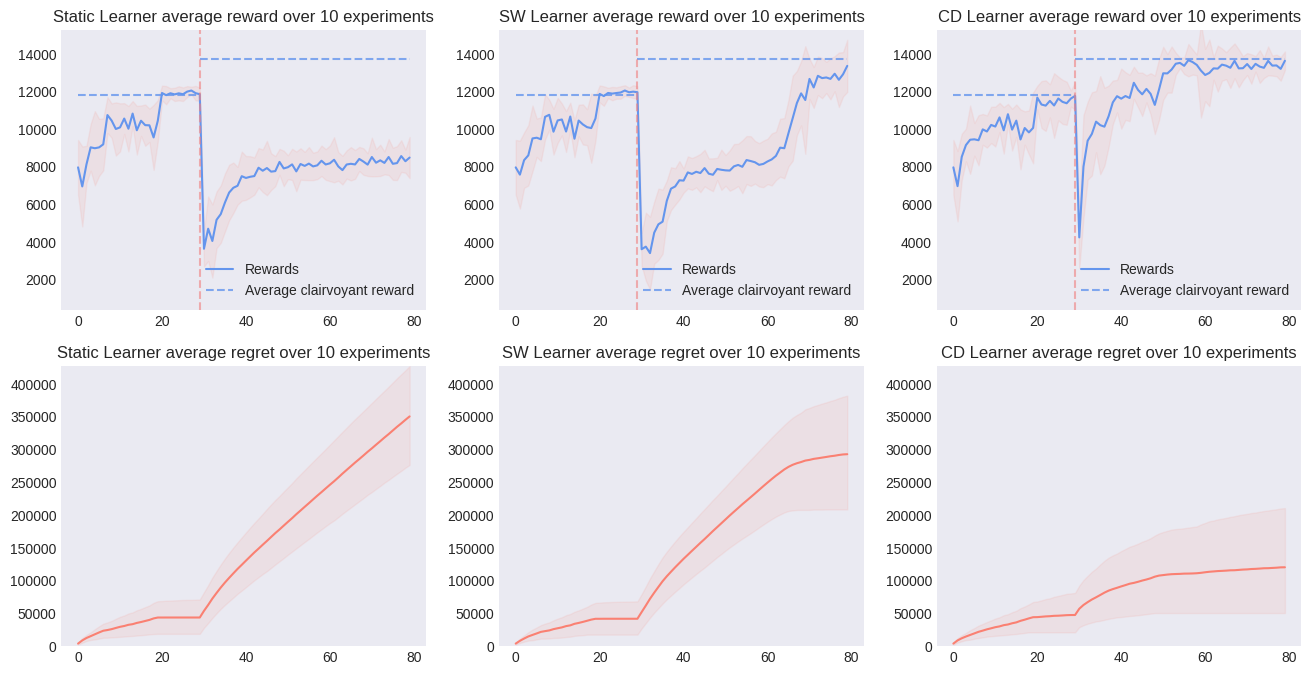
\includegraphics[scale=0.32]{img/Graphs/non_stationary/image4.png}
\end{center}

\scriptsize All tests are done using the \texttt{example\_environment} with default values, \textit{population mean} of 1000, \textit{variance} of 10 and 20 \textit{budget steps}. Only \textbf{UCB} algorithms were evaluated. 1 breakpoint at 30 days.

\end{frame}

% ----------------------------------------

\begin{frame}
\frametitle{Results}

From the results it's quite clear that the \textbf{change detection} algorithm is by far the best one in this specific scenario, while it's interesting to see that the \textbf{sliding window} approach it's slower to stabilize (due to the fact that the samples from the old environment must completely exit the window to not be considered) and the \textbf{base learner} approach isn't able to adapt, as expected.

Generalizing, we can say that if the \textbf{number of breakpoints} $m$ is small enough with respect to the \textbf{time horizon} $T$ to the power of $\alpha$ we have that the \textbf{regret} is of the order $O\left( \vert A \vert T^{\frac{1+\alpha}{2}} \right)$.

\end{frame}

% ----------------------------------------

\begin{frame}
\frametitle{Results}

Average results over 10 runs at time horizon $T = 80$:

\begin{table}
    \begin{tabular}{|c|cc|c|}
    \hline \hline
        \cellcolor{blue!25} & Reward 	& Regret	& Deviation \\
    \cline{2-4}
        \cellcolor{blue!25} & $\mu$		& $\mu$		& $\sigma$	\\
    \hline \hline
        Base learner		& 7717.40	& 376073.10	& 877.73	\\
    \hline
        Sliding window		& 12571.80	& 271383.60	& 908.26	\\
    \hline
        Change detection	& 13452.30	& 126329.10	& 684.53	\\
    \hline \hline
    \end{tabular}
\end{table}

\end{frame}

% ----------------------------------------
